\chapter{Executive Summary}

In this penetration test the Company X was examined for security-relevant weaknesses. The kind of testing was black-box, this is the kind where no specific information about the internals of the system is given. The scope of the assessment was as follows:
\begin{itemize}
	\item Dedicated Web Server: 127.0.0.1
	\begin{itemize}
		\item Domain: https://example.com
		\begin{itemize}
			\item Subdomains: all subdomains
		\end{itemize}
	\end{itemize}
\end{itemize}

Table \ref{tbl:web-sites} contains the overview of examined systems during the penetration test.
\begin{table}[h]
	\centering
	\begin{tabular}{|l|l|}
		\hline 
		\textbf{Web Site} & \textbf{Hostname}\\
		\hline 
		Domain 1 & https://example.com/\\
		\hline 
		Subdomain 1 & https://1.example.com/\\
		\hline 
		Subdomain 2 & https://2.example.com/\\
		\hline 
	\end{tabular}
	\caption{Web sites examined during the penetration test}
	\label{tbl:web-sites}
\end{table}

As a result, several vulnerabilities have been found among the assets of the organization, some of them pose a significant risk. Figure \ref{fig:vuln-by-type} summarizes all issues by their type across all the assets of Company X. Solutions to remedy the discovered vulnerabilities are provided together with detailed descriptions and reproduction steps.

\begin{figure}[h]
	\centering
	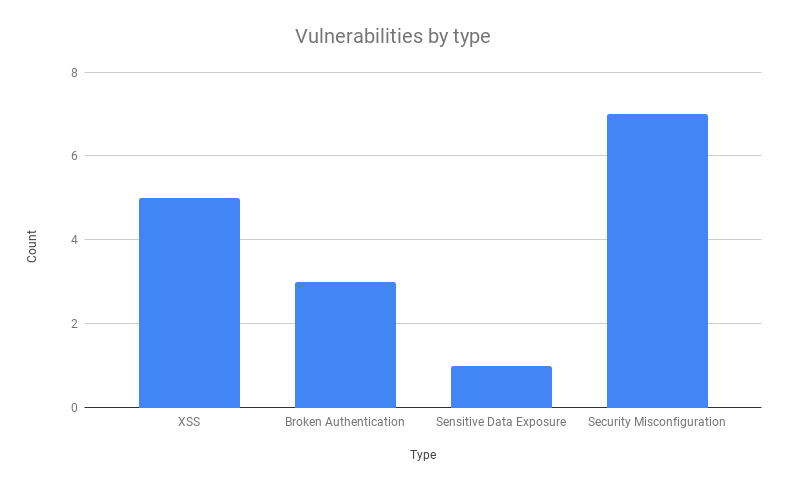
\includegraphics[width=0.6\textwidth]{img/vulns-by-type.png}
	\caption{Vulnerabilities by Type}
	\label{fig:vuln-by-type}
\end{figure}

In this part add a short summary of all vulnerabilities in non-technical terms.

It's also good to mention an estimation of efforts required to resolve the issues.